\chapter{Sujet de stage}
D’un point de vue technique l’équipe de lesfurets.com a décidé d’abstraire les champs du formulaire ainsi que les dépendances à l’aide d'un metamodel. C'est à dire que les champs ainsi que leurs dépendances épousent un format défini à un niveau d'abstraction diffèrent du code. Ils ne sont pas implémentés au moment de l'instanciation des champs mais au niveau du modèle de données sous forme d'Enum Java. L'implantation de la construction permet de caractériser chaque champ et de le présenter à l'utilisateur sous la forme voulu (combo box, radio bouton, date picker, ...). De plus chaque champ connaîtrait par la suite les comportement nécessaires lors de l'évolution de ses co-dépendants.  A l’heure actuelle, l’application Web est capable de transformer ce modèle de champs au format XMI pour pouvoir l'exporter dans un logiciel de modélisation comme MagicDraw, Rational. Le stage débutera par un passage à d’autres formats de modélisation (EMF, JSON) traités à l'aide d'outils open-source qui permettront aux équipes de mieux visualiser le graphe des champs des formulaires ainsi que leurs dépendances. Il est prévu ensuite de superposer des trackers analytics sur ces graphes. Il est aussi envisagé de garder une trace des différences entre les versions successives de l’application pour visualiser les modifications et/ou les régressions en fonctions des développements. Enfin au même titre qu’un IDE classique, l’outil devrait pouvoir proposer des fonctions d’édition, de sauvegarde et de partage des données traitées.

\section{Metamodel}
Metamodel signifie littéralement modèle du modèle. Il peut être défini comme la représentation d'un point de vue particulier sur des modèles. On peut voir les couches d'abstraction entre le modèle et le metamodel. Certains langages à objets, comme Java, décrivent de la même manière les classes, les métaclasses et les objets. En génie logiciel, c'est avec UML que la notion de métamodèle a été développée. Le métamodèle décrit les modèles : classes, objets, attributs, relations… et se décrit lui-même. Au-delà de leur diversité, les modèles présentent une caractéristique commune : ils sont des représentations d’un point de vue (d'une conception, d'une théorie…) particulier sur un système sujet d’études. Ils sont écrits dans un code (un langage, un formalisme…) approprié à l'expression et à l'usage des connaissances qu'ils véhiculent.
La notion de « Modèle » est donc directement liée à celles de « Formalisme », de « Point de Vue/Théorie » et de « Sujet d'étude/Système ». On retrouvera l'application de la notion de model et de metamodel dans la figure ci-dessous.
\begin{figure}[!h]
\centering
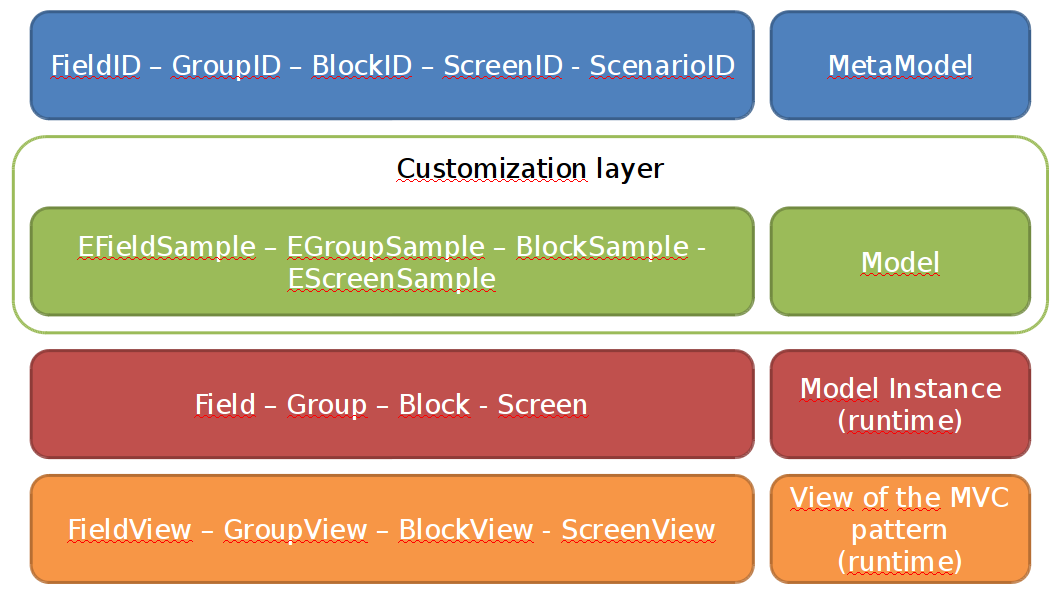
\includegraphics[width=15cm]{sujet/metamodel.png}
\caption{Modele et Metamodel appliqué aux formulaires du site}
\end{figure}

\section{Analyse du metamodel}
Le metamodel étant déjà exploiter dans l'application sous un format exportable, ma première approche était d'afficher le modèle du formulaire pour trouver un moyen pertinent de l'afficher par la suite. Il m'a fallu me familiariser avec l'outil de modeling déjà utilisé dans l'entreprise : MagicDraw. Le diagramme UML présenté montre des cycles, rares mais présent, dans le graphe de dépendances. Le données peuvent être des "fields", "groups", "blocks" ou "screen" ce qui correspond respectivement à un champ du formulaire, un groupe de champs, un bloc de champs et un écran. Pour avoir une vision plus concrète de leur correspondance dans un formulaire du site vous pouvez voir dans l'image ci-dessous que nous sommes dans l'écran "Votre Véhicule", dans le bloc "Ma demande", qu'il existe un groupe pour la recherche du véhicule, en fonction de la marque et du modèle, regroupant plusieurs champs.  De plus il existe une hiérarchie claire dans le graphe. Tous les champs, bloc et groupe sont compris dans un écran, les champs peuvent être compris dans un blocs ou groupe et les groupe peuvent être compris dans un bloc. Chaque groupe, bloc ou écran comporte au moins champ. Tous les éléments sont regroupés au sein d'Enum Java
\begin{center}
\vspace{0.5cm} 
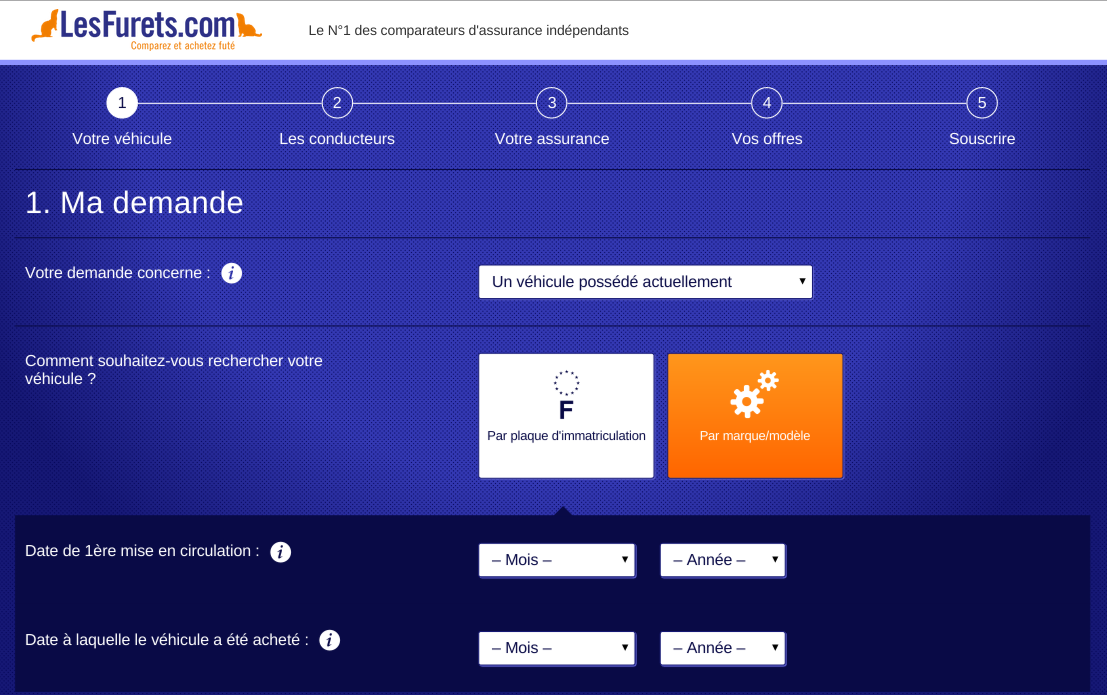
\includegraphics[height=10cm]{fields.png}
\end{center}

\begin{lstlisting}[caption=Enum Java de l'écran Véhicule]
public enum EScreenAuto implements ScreenID, CodeLookup<EScreenAuto> {

    SCR_VEHICULE("Vehicule", ID_STAT_VEHICULE, PRE_TARIFICATIONS, //
                    BLK_MA_DEMANDE, //
                    BLK_UTILISATION_DU_VEHICULE, //
                    GRP_QUOTE),
\end{lstlisting}

\begin{lstlisting}[caption=Enum Java du bloc Ma Demande]
public enum EBlockAuto implements BlockID, CodeLookup<EBlockAuto> {

    // Votre véhicule
    BLK_MA_DEMANDE("BLK_MA_DEMANDE", //
                    ID_STAT_VEHICULE, //
                    VEH_DTL_DEMANDE, //
                    VEH_DTL_CHOIX_RECHERCHE_VEHICULE,//
                    GRP_VEH_IMMAT, //
                    GRP_VEH_ETAT_FINANCE, //
                    GRP_VEH_IMMAT_ACHAT_ACHAT_PREVU, //
                    VEH_DTL_SELECTION_MODELE, //
                    VEH_DTL_CODE_SRA, //
                    VEH_DTL_VALEUR_REELLE, //
                    VEH_DTL_VALEUR_ESTIMEE, //
                    VEH_DTL_TITULAIRE, //
                    VEH_DTL_SECOND), //
\end{lstlisting}

\begin{lstlisting}[caption=Enum Java du groupe choix du modèle]
public enum EGroupAuto implements GroupID, CodeLookup<EGroupAuto> {
    GRP_VEH_ETAT_FINANCE("GRP_VEH_ETAT_FINANCE", //
                    VEH_DTL_ETAT), //
    GRP_VEH_IMMAT("GRP_VEH_IMMAT", //
                    VEH_DTL_IMMAT_NUM,//
                    VEH_DTL_IMMAT_SERVICE,//
                    VEH_DTL_IMMAT_DESCRIPTIONS,//
                    VEH_DTL_IMMAT_REGISTRATION,//
                    VEH_DTL_IMMAT_VERSIONS),//
    GRP_VEH_VEHICULE_MOBILE("GRP_VEH_VEHICULE_MOBILE", //
                    VEH_DTL_VEHICULE_TITRE, //
                    VEH_DTL_AVAILABLES, //
                    VEH_DTL_MODE_CAROSSERIE, //
                    VEH_DTL_MARQUE, //
                    VEH_DTL_MODELE, //
                    VEH_DTL_CARBURANT, //
                    VEH_DTL_CARROSSERIE, //
                    VEH_DTL_PUISSANCE, //
                    VEH_DTL_VERSION), //
    GRP_VEH_IMMAT_ACHAT_ACHAT_PREVU("GRP_VEH_IMMAT_ACHAT_ACHAT_PREVU", //
                    VEH_DTL_IMMAT, //
                    VEH_DTL_ACHAT, //
                    VEH_DTL_ACHAT_PREVUE), //
\end{lstlisting}
\clearpage
\section{Analyse Fonctionnelle}
Les utilisateurs de l’outil seront d’une part les architectes logiciel de la société, les développeurs mais aussi les Business Analysts (concepteurs fonctionnels) qui pourront mieux cerner les impacts des modifications au seins du formulaire. Ils pourront aussi mieux cibler les besoin des utilisateurs du site. Ainsi il faudra imaginer une interface qui pourrait s'apparenter à des wireframes qui ne sera plus l’apanage des seuls ingénieurs. On pourrait aussi proposer des interfaces différentes en fonctions des utilisateurs de l'outil et de l'utilisation qu'ils en feront.

\section{Conception}
Dans le cadre du projet, il me faudra explorer plusieurs pistes :
La première consistera à me familiariser avec un outil de modeling basé sur Eclipse : Sirius (https://eclipse.org/sirius/overview.html). Sirius est un projet Open Source de la Fondation Eclipse. Cette technologie permet de concevoir un atelier de modélisation graphique sur-mesure en s'appuyant sur les technologies Eclipse Modeling, en particulier EMF et GMF. L'atelier de modélisation créé est composé d'un ensemble d'éditeurs Eclipse (diagrammes, tables et arbres) qui permettent aux utilisateurs de créer, éditer et visualiser des modèles EMF. Le projet est une initiative française et la communauté autour du projet est très active. Je me mettrai en relations avec les créateurs du projet pour pouvoir aborder les questions que j’aurai tout au long de mon stage.
Il me faudra aussi explorer la piste de la création d'une application Web en charge d’afficher le modèle. Il existe de multiple librairies en JavaScript pour l’affichage des données sous la forme de graphe orienté. De plus il s'agit d'un graphe orienté faiblement cyclique qu'on pourra traiter, coté serveur avec des algorithmes implémenté en Java, Scala, Python ou JavaScript. Enfin aujourd’hui le graphe est généré sur un fichier au format XMI mais on pourrai imaginer que l’outil introspecte les objets directement dans les binaires. De plus, étant donnée l'étendue de la problématique, la solution pourrait se répartir sur plusieurs outils.

\section{Fonctionnalités futures}
Une fois l’outil développé et adapté aux besoins des formulaires, les équipes souhaiteraient aussi modéliser d'autres données déjà représentées par des metamodels au sein de l'application Java.

\subsection{Page du site}
Les pages du site, les URL, les CSS, ainsi que la JSP utilisés sont représentés dans l'application sous forme d'Enum Java. Ainsi au même titre que pour les champs du formulaire on pourrait imaginer un outil affichant une carte des pages du site ainsi que leurs liens les unes vers les autres. Nous pourrions par la suite lier les données SEO déjà présentes et les afficher à même le graphe.

\subsection{CRM - Envoi d'emails}
Les site communique avec ses utilisateurs grâce à des emails envoyés une fois leur parcours fini. Par exemple une fois un formulaire rempli si aucune offre n'est choisi l'utilisateur peut choisir de recevoir des offres en fonction des critères qu'il a choisi. C'est ainsi que l'application gère un nombre de règle pour un envoi d'email automatique à différents moments du cycle de vie d'une fiche utilisateur.
Ce modèle d'email est lui aussi abstrait grâce à un metamodel et un modèle de donnée défini dans une Enum Java. On pourrait, comme pour les champs des formulaires, imaginer de modéliser le cycle de vie d'une fiche utilisateur avec le nombre d'envois d'emails, les dates ; et superposer les données de retour des utilisateurs en fonction des mails envoyé.